\documentclass{article}
\usepackage{amsmath}

\usepackage{full page}  % make the margins somewhat smaller than the default

\usepackage{listings}  %  needed for source code listings
\usepackage{color}
\usepackage{hyperref}
\usepackage{graphicx}
\usepackage{caption}
\usepackage{subcaption}
\usepackage{float}

\graphicspath{ {Images/} }

\definecolor{javared}{rgb}{0.7,0,0} % for strings
\definecolor{javagreen}{rgb}{0.25,0.6,0.35} % comments
\definecolor{javapurple}{rgb}{0.55,0,0.40} % keywords
\definecolor{javadocblue}{rgb}{0.25,0.35,0.85} % javadoc
 
\lstset{language=Java,
basicstyle=\ttfamily,
keywordstyle=\color{javapurple}\bfseries,
stringstyle=\color{javared},
commentstyle=\color{javagreen},
morecomment=[s][\color{javadocblue}]{/**}{*/},
numbers=left,
numberstyle=\tiny\color{black},
stepnumber=2,
numbersep=10pt,
tabsize=2,
showspaces=false,
showstringspaces=false,
frame=shadowbox,
numbers=left
} 

% set the document title, author, and date here.
%  once set, the \maketitle command (within the document)
%  will display them nicely
\title{AI Assignment 4 - Chess Game}
\author{Tianyuan Zhang}

\begin{document}
\maketitle

\section{Introduction}
The adversarial search in Zero-Sum games is an important area of AI, which can also be applied to many real world applications also. The Chess game is the representative among these games. In this assignment I build a Chess AI and tried to optimize it in terms of time and space. In this assignment, I implemented the Minimax Method, Alpha-Beta Pruning, Transposition table, Profile Analysis and Move reordering.

\section{Minimax Search}
\subsection{Basic Idea}
The basic idea of Minimax Search is that whenever we need to make a decision in a game, we are not only evaluate according to the current state of the game, but also the opponent's play - the reaction of adversary in his/her turn. As it is obviously a tree shape prediction model, we can use computer to process the tree and try to find the best movement for the current player according to the prediction for the next few moves. In Minimax Search algorithm, the current play always want its score to be maximum, while its opponent always want its score to be minimum. Then for each level of the prediction tree we have a evaluation for each node corresponding to the current player, so basically we just enumerate all the possible moves of the whole game. However as the limitation of the computation power of the computer, we need to limit the max-depth of the search tree and pick the best move found so far.

\subsection{Code Implementation}
\subsubsection{Class : MoveVal}
This class helps store the move-evaluation pair.
\begin{lstlisting}
public class MoveVal{
	private short move;
	private int val;
	
	public MoveVal(){
		move = 0; val = 0;
	}
	public MoveVal(short m, int v){
		move = m; val = v;
	}
	public void setVal(int v){val = v;}
	public void setMove(short m){move = m;}
}
\end{lstlisting}
\subsubsection{minimaxIDS}
This method is theiterative deepening returns a $short$ type result which represents the next best move for the current player. This method will call mthod $maxMove$.
\begin{lstlisting}
private short miniMaxIDS(Position position, int maxDepth) 
			throws IllegalMoveException{
	MoveVal bestMove = new MoveVal();
	for(int i = maxDepth - 1; i >= 0; i--)
		bestMove = maxMove(position, i);
	return bestMove.move;
}
\end{lstlisting}

\subsubsection{maxMove}
This method is the $Max$ part of the Maxmini Seerch. For a given position of the current player, this method try each possible move for the next player and call $minMove$ method to get the evaluation of the oponent, then according to the evaluation of the opponent to choose the best move for the current player.
\begin{lstlisting}
private MoveVal maxMove(Position position, int depth) 
		throws IllegalMoveException{
	MoveVal bestMove = new MoveVal((short) 0, Integer.MIN_VALUE);
	if(depth == max_depth || position.isTerminal()){
		bestMove.setMove(position.getLastShortMove());
		bestMove.setVal(utility(position));
	} else{
		for(short move : position.getAllMoves()){
			position.doMove(move);
			int val = (minMove(position, depth + 1)).val;
			if(bestMove.val < val){
				bestMove.setVal(val);
				bestMove.setMove(move);
			}
			position.undoMove();
		}
	}
	return bestMove;	
}
\end{lstlisting}

\subsubsection{minMove}
This method is the $Min$ part of the Maxmini Search. It will get the position from the method $maxMove$ and call $maxMove$ for each possible next move. Then it will chose the minimum evaluation among all the evaluation it gets.
\begin{lstlisting}
private MoveVal minMove(Position position, int depth) 
		throws IllegalMoveException{
	MoveVal bestMove = new MoveVal((short)0, Integer.MAX_VALUE);
	if(depth == max_depth || position.isTerminal()){
		bestMove.setMove(position.getLastShortMove());
		bestMove.setVal(utility(position));
	} else {
		for(short move : position.getAllMoves()){
			position.doMove(move);
			int val = (maxMove(position, depth + 1)).val;
			if(bestMove.val > val){
				bestMove.setMove(move);
				bestMove.setVal(val);
			}
			position.undoMove();
		}
	}
	return bestMove;
}
\end{lstlisting}

\subsubsection{utility}
This method is for handling the terminal. When the tree reaches the max-depth or reaches a draw or check mate, it will return the corresponding evaluation.
\begin{lstlisting}
private int utility(Position position){
	if(position.isTerminal() && position.isMate()){
		if(position.getToPlay() == curPlayer)
			return Integer.MIN_VALUE;
		else return Integer.MAX_VALUE;
	}
	else if(position.isTerminal()) return 0;
	else{
		int value = position.getMaterial() + (int)position.getDomination();
		if(curPlayer == position.getToPlay())
			return value;
		else return -value;
	}
}
\end{lstlisting}

\subsection{Result}
Here I would like to show two experiments I played with the Maximini Search AI. I set up two games, both of them are Minimax AI v.s. Random AI, but one of them is with max-depth = 1 and another one is with max-depth = 3. The difference between the decision that the AI made is obvious.
\clearpage
\subsubsection{max-depth = 1}
This AI plays like a Chess newbie - it always want to capture the oponent whenever possible. The result is that it can always win the random AI but it will spend a lot of steps. The result shown as follow, we can see that the random AI (Black) has almost nothing left and it cost Minimax AI (White) 19 turns to win.

\begin{lstlisting}
White Wins!
making move 7534
N4k2/5Q2/2P1B3/7p/3P1p2/P4P2/P1P3PP/R3K1NR b KQ - 1 19
\end{lstlisting}
\begin{figure}[H]
\centering
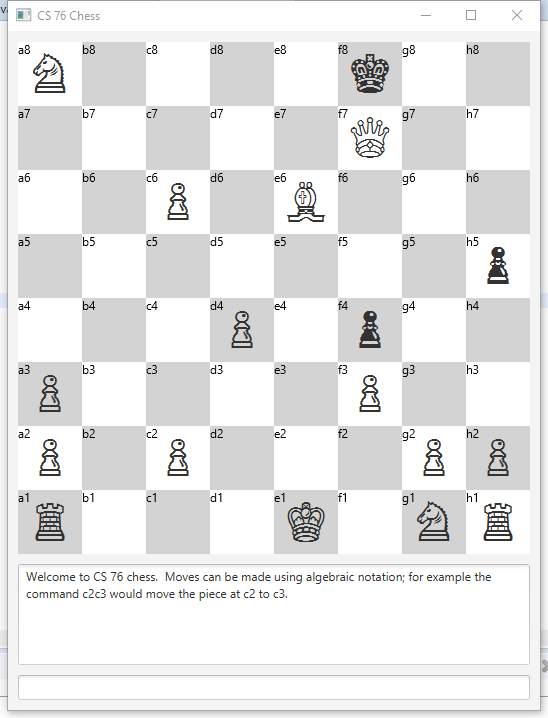
\includegraphics[width=0.7\linewidth]{max_1_rnd}
\caption{Minimax(depth = 1) AI vs Rnd AI}
\end{figure}

\clearpage
\subsubsection{max-depth = 3}
This AI plays smarter - it may not capture as many as the AI with depth = 1, but it can always win quick. We can see that White only capture one Pawn but wins in 8 turns.
\begin{lstlisting}
White Wins!
making move -25251
rnbqk2r/2pp1Q1p/pp1bp1p1/3nP1N1/8/2N5/PPPP1PPP/R1B1KB1R b KQkq - 0 8
\end{lstlisting}

\begin{figure}[H]
\centering
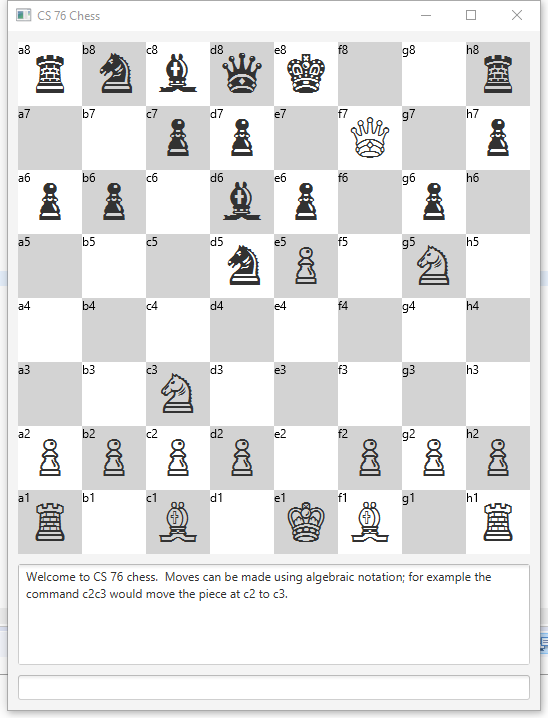
\includegraphics[width=0.7\linewidth]{max_3_rnd}
\caption{Minimax(depth = 3) AI vs Rnd AI}
\end{figure}

\section{Alpha-Beta Pruning}
\subsection{Basic Idea}
The basic idea of Alpha-Beta Pruning is to prevent traversal the branch of the tree as much as possible. For the AB Pruning, it will records the current minimum evaluation and maximum evaluation for the node and if the next step is obviously worse than the current step, then we can prevent traversal that branch.

\subsection{Code Implementation}
Basically the implementation of AB Pruning is a lot like the Minimax Search except that the Alpha-Beta constraints are added.
\subsubsection{maxMove}
The difference is that lines 16-20 are added to jump out of the loop earlier if possible.
\begin{lstlisting}
	private MoveVal maxMove(Position position, int depth, int alpha, int beta) throws IllegalMoveException {
		MoveVal bestMove = new MoveVal((short) 0, Integer.MIN_VALUE);
		if (depth == max_depth || position.isTerminal()) {
			bestMove.setMove(position.getLastShortMove());
			bestMove.setVal(utility(position));
		} else {
			for (short move : position.getAllMoves()) {
				position.doMove(move);
				int val = (minMove(position, depth + 1, alpha, beta)).val;
				if (bestMove.val < val) {
					bestMove.setVal(val);
					bestMove.setMove(move);
				}
				position.undoMove();
				alpha = bestMove.val;
				if (alpha >= beta) {
					bestMove.setVal(beta);
					break;
				}
			}
		}
		return bestMove;
	}
\end{lstlisting}

\subsubsection{minMove}
The difference is that lines 16-20 are added to jump out of the loop earlier if possible.
\begin{lstlisting}
	private MoveVal minMove(Position position, int depth, int alpha, int beta) 
			throws IllegalMoveException {
		MoveVal bestMove = new MoveVal((short) 0, Integer.MAX_VALUE);
		if (depth == max_depth || position.isTerminal()) {
			bestMove.setMove(position.getLastShortMove());
			bestMove.setVal(utility(position));
		} else {
			for (short move : position.getAllMoves()) {
				position.doMove(move);
				int val = (maxMove(position, depth + 1, alpha, beta)).val;
				if (bestMove.val > val) {
					bestMove.setMove(move);
					bestMove.setVal(val);
				}
				position.undoMove();
				beta = bestMove.val;
				if(beta <= alpha){
					bestMove.setVal(alpha);
					break;
				}
			}
		}
		return bestMove;
	}
\end{lstlisting}

\subsection{Result}
For this part I majorly want to show the correctness of my AB Pruning implementation and the better performance of AB Pruning over Minimax Search.
\subsubsection{Correctness}
To check the correctness of the AB Pruning implementation is that given the same situation, AB Pruning should perform the same moves as Minimax Search. So my method is to first let a White(Minimax with depth = 3) vs Black(ABP with depth = 3), then let a White(ABP with depth = 3) vs Black(Minimax with depth = 3). If my AB Pruning was right, then the result of these two playes should be excatly the same. The results shows that though I switch two AI's position, the winner is always the White side with 29 turns and with the same ending position. Here is the result:

\clearpage
\textbf{White(Minimax) vs Black(ABP)}
\begin{lstlisting}
White Wins!
making move 7030
1Bbkq2r/1p3p1p/3p1Q2/2pP4/5P2/2P5/P5PP/2KnR3 b - - 1 29
\end{lstlisting}

\begin{figure}[H]
\centering
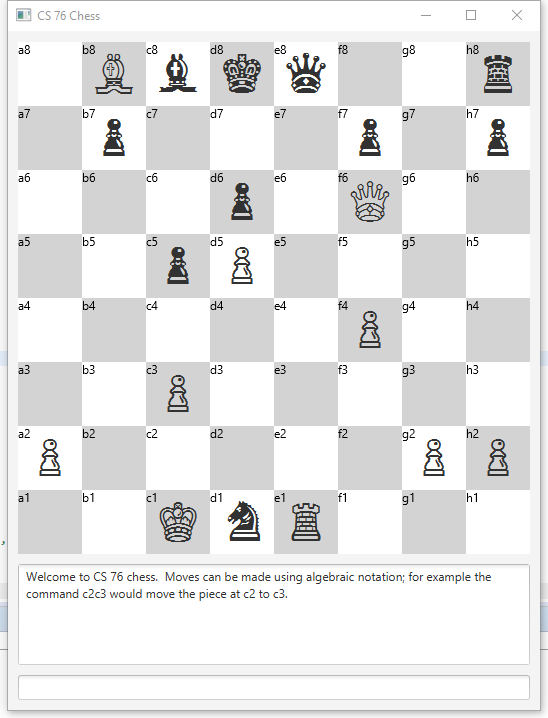
\includegraphics[width=0.7\linewidth]{W_MINI_B_ABP}
\caption{White(Minimax) vs Black(ABP)}
\end{figure}

\clearpage
\textbf{White(ABP) vs Black(Minimax)}
\begin{lstlisting}
making move 7030
1Bbkq2r/1p3p1p/3p1Q2/2pP4/5P2/2P5/P5PP/2KnR3 b - - 1 29
White Wins!
\end{lstlisting}

\begin{figure}[H]
\centering
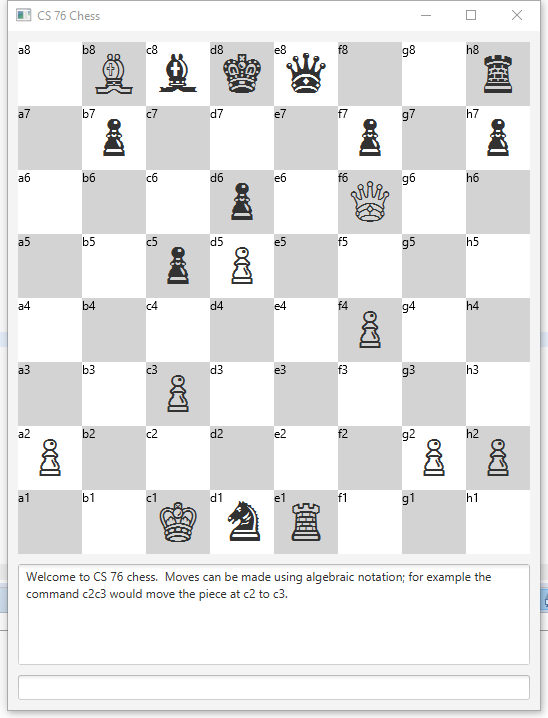
\includegraphics[width=0.7\linewidth]{W_ABP_B_MINI}
\caption{White(ABP) vs Black(Minimax)}
\end{figure}

\subsubsection{Performance}
To show that the performance of AB Pruning is better than Minimax Search, I also set up two plays - one is Minimax v.s. Minimax and another one is Minimax v.s. ABP. All the AI have the sampe max-depth = 3. By showing the total time each play spend, we can see that AB Pruning is actually beat Minimax in terms of performance. Here is the result:

\end{document}